\documentclass[tikz,border=10pt]{standalone}
% https://tex.stackexchange.com/q/755422/322482
\def\totalwidth{10}
\def\totalheight{3.5}
\def\mysep{0.3}
\def\splitratio{0.98}

\newcommand\recursivenodes[6]{%
    % #1: Depth
    % #2: Width
    % #3: Height
    % #4: X coordinate
    % #5: Y coordinate
    % #6: Scale
    \begingroup
    \pic[scale=#6,transform shape] at (#4,#5) {offtopic};
    \ifnum#1>1\relax
        \pgfmathtruncatemacro{\nextdepth}{#1-1}
        \pgfmathsetmacro{\xoffset}{(.5-.25*\splitratio)*#2}
        \pgfmathsetmacro{\nextwidth}{.5*\splitratio*#2}
        \edef\tmph{#3}
        \pgfmathsetmacro{\nextheight}{.5*\splitratio*\tmph}

        \pgfmathsetmacro{\nexty}{#5 - .5 * \tmph - .5 * \nextheight - \mysep * \nextdepth * .15 }
        \edef\tmpx{#4}

        \pgfmathsetmacro{\leftx}{\tmpx - \xoffset}
        \pgfmathsetmacro{\rightx}{\tmpx + \xoffset}

        \pgfmathsetmacro{\nextscale}{.5*\splitratio*#6}
        % Left subtree
        \recursivenodes{\nextdepth}{\nextwidth}{\nextheight}{\leftx}{\nexty}{\nextscale}
        % Right subtree
        \recursivenodes{\nextdepth}{\nextwidth}{\nextheight}{\rightx}{\nexty}{\nextscale}
    \fi
    \endgroup
}

% https://tex.stackexchange.com/a/755485/322482
\makeatletter
\newcommand{\calcscaling}{
  \pgfgettransformentries{\tmpscaleA}{\tmpscaleB}{\tmpscaleC}{\tmpscaleD}{\tmp}{\tmp}%
  \pgfmathsetmacro{\scalingfactor}{sqrt(abs(\tmpscaleA*\tmpscaleD-\tmpscaleB*\tmpscaleC))*sqrt(abs((\pgf@xx/1cm)*(\pgf@yy/1cm)-(\pgf@xy/1cm)*(\pgf@yx/1cm)))}%
}
\makeatother

\begin{document}
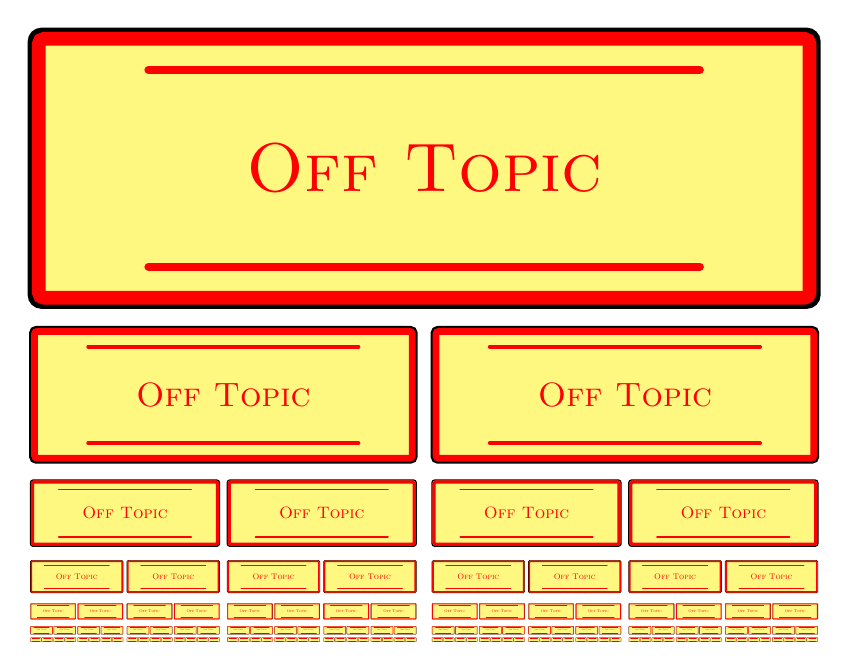
\begin{tikzpicture}[
        offtopic/.pic={%
            \calcscaling%
            \node[%
                draw,fill=yellow!50,
                line width=\scalingfactor*2pt,
                rounded corners=\scalingfactor*4pt,
                text=red,font=\scshape\Huge,
                minimum width=\totalwidth cm,
                minimum height=\totalheight cm, 
                inner sep=0pt,
                outer sep=0pt,
            ] (tmp) {Off Topic};
            \draw[red,line cap=round,line width=\scalingfactor*3pt] ([shift={(1.5cm,-.5cm)}]tmp.north west) -- ([shift={(-1.5cm,-.5cm)}]tmp.north east);    
            \draw[red,line cap=round,line width=\scalingfactor*3pt] ([shift={(1.5cm,.5cm)}]tmp.south west) -- ([shift={(-1.5cm,.5cm)}]tmp.south east);
            \draw[red,ultra thick,rounded corners=\scalingfactor*2pt,line width=\scalingfactor*5pt] 
            ([shift={(3pt,-3pt)}]tmp.north west) 
            rectangle 
            ([shift={(-3pt,3pt)}]tmp.south east)
            ;
        }
    ]
    \recursivenodes{7}{\totalwidth}{\totalheight}{0}{0}{1}

\end{tikzpicture}
\end{document}
